\documentclass{beamer}
\usepackage[utf8]{inputenc}
% \usepackage{default}
% \usepackage{paralist}
% \usepackage{enumitem}
\usepackage{changepage}
\usepackage{enumerate}
% \setlist{align=left}
% \usetheme{Antibes}
\usetheme{Warsaw}
\geometry{paper=a4}
\def\Put(#1,#2)#3{\leavevmode\makebox(0,0){\put(#1,#2){#3}}}

\title{PATENA: an algorithm for the design of protein linker sequences}
\date{}

\author{Ignacio Eguinoa, Ignacio Enrique Sánchez}
\institute[VFU] % (optional)
{ Protein Physiology Laboratory, Departamento de Química Biológica, Facultad de Ciencias Exactas y Naturales and IQUIBICEN-CONICET, Universidad de Buenos Aires, Buenos Aires, Argentina}

\begin{document}

\begin{frame}
 \titlepage
\end{frame}

\section{Intro}

\begin{frame}{Chimeric proteins}
\Put(160,0){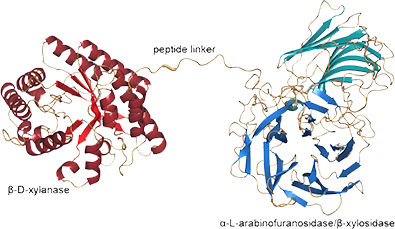
\includegraphics[width=150px]{../img/fusionEnzymes.png}}
\begin{itemize}
% use of protein engineering process to covalently join 2+ proteins/domains
 \item Join 2+ proteins/domains  
 \vspace{20px}
 \pause
 \item Function arising from linked subunits
 \pause
 \vspace{20px}
% \Put(0,0){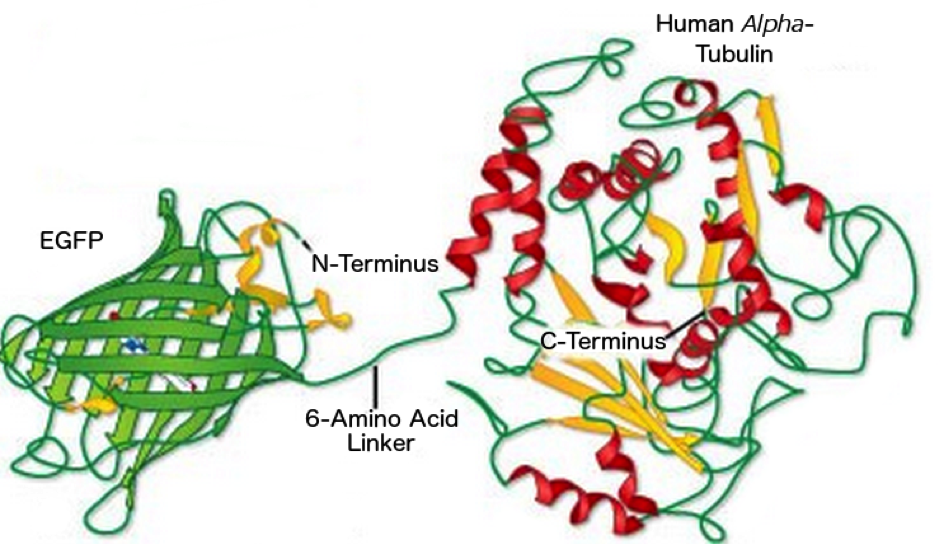
\includegraphics[width=120px]{../img/gfp.png}}
\makebox(0,0){\put(0,-170){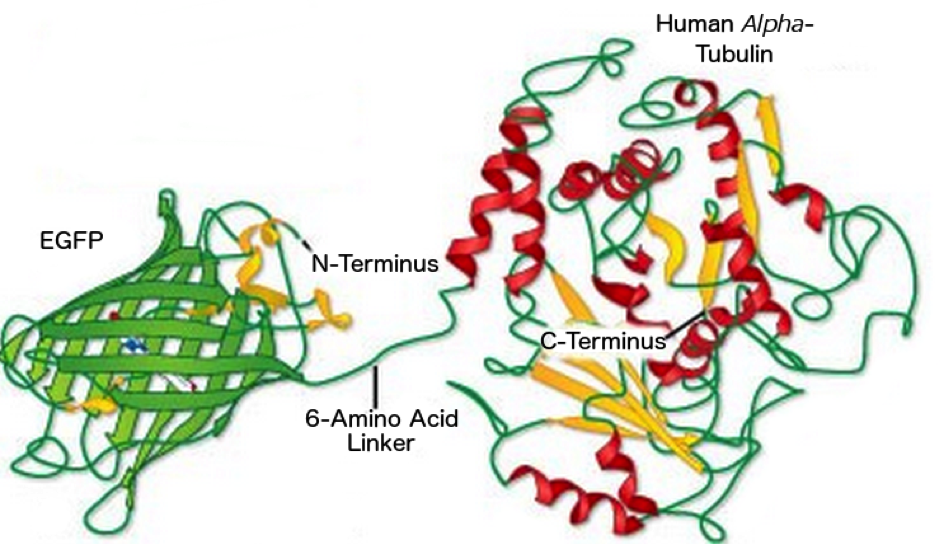
\includegraphics[width=140px]{../img/gfp.png}}}
\item Wide range of applications
\end{itemize}
\vspace{30px}
\Put(0,10){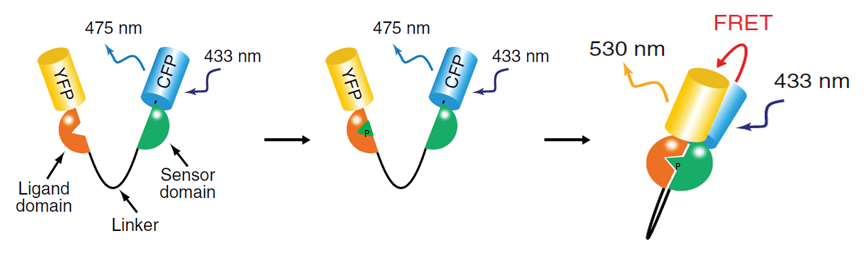
\includegraphics[width=170px]{../img/fret.png}}
% \hspace{150px}


% QUE SON
% ejemplos:
% 	Formación de proteinas bifuncionales mediante union covalente de dominios.
% 	Promover la unión entre proteinas que forman complejos, generando una unión covalente entre ellos
% 
% proceso de sintesis:
% 	-unir los dominios de interes
%       -clone into expression system
\end{frame}




\begin{frame}{Chimeric proteins}
What we need:
\begin{itemize}
 \item 2+ proteins/domains
 \item Linker sequence
%  por que es necesario???
% The construction of a multifunctional enzyme by simple head-to-tail fusion of parental  enzymes  often  results  in  non-functional  enzymes
% because of either incorrect folding or restrained ability to interact with other protein subunits (Hua et al., 2004)
 \begin{itemize}
    \pause
    \item Allows domains to fold independently, move and interact freely
%  \subitem Keep domains together so they work as a unit
\end{itemize}
\end{itemize}
% 
\includegraphics[width=10px]{../img/okMark.png}
% \hspace*{100px}
\vspace{20px}
% 
\includegraphics[width=10px]{../img/xMark.png}
\pause
\hspace{20px}
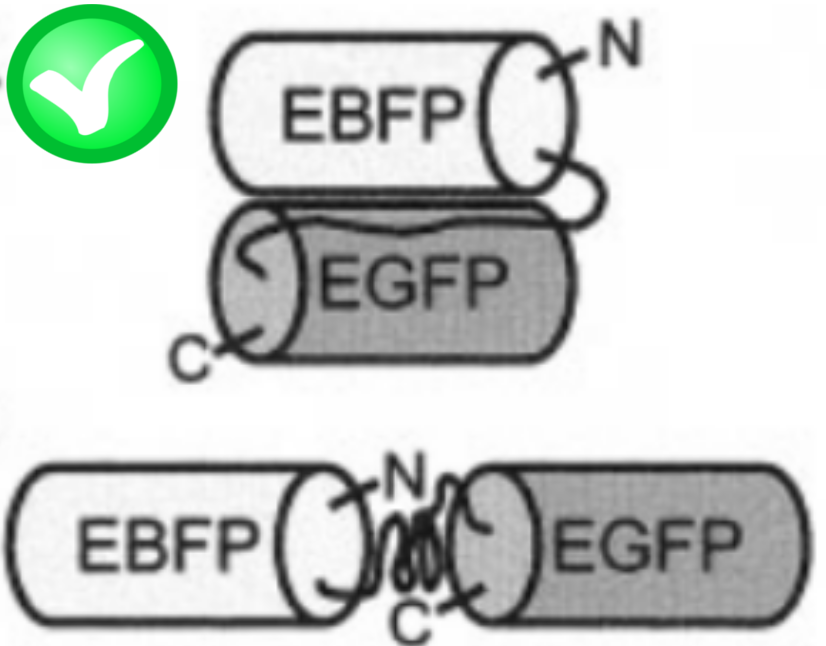
\includegraphics[width=100px]{../img/linkerOk-sign.png}
\hspace{40px}
\pause
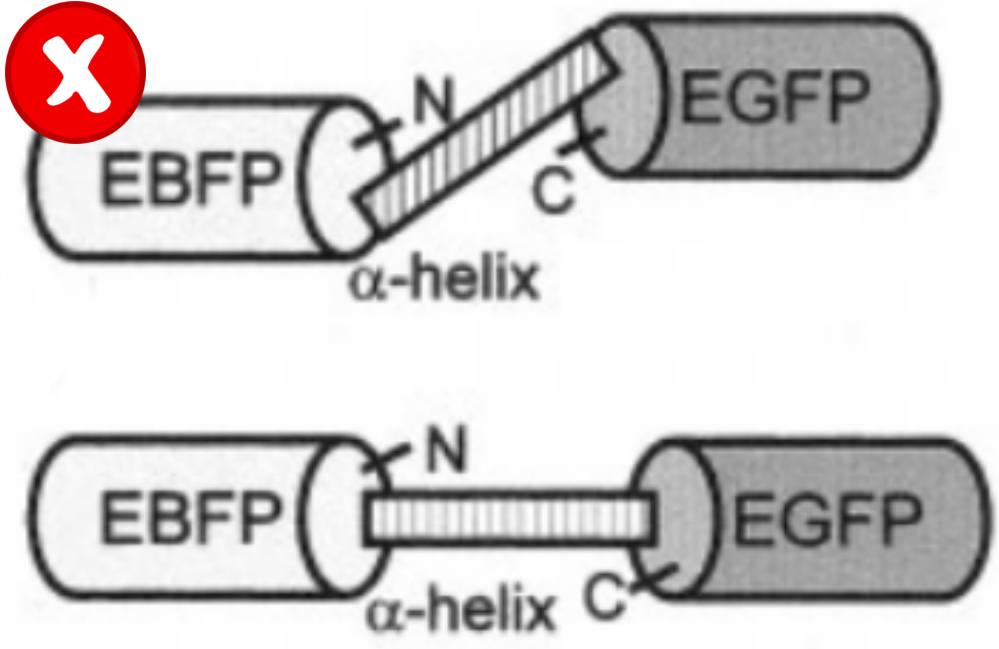
\includegraphics[width=120px]{../img/linkerBad-sign.png}
\end{frame}



% 
% \begin{frame}[plain]
% \begin{center}
% 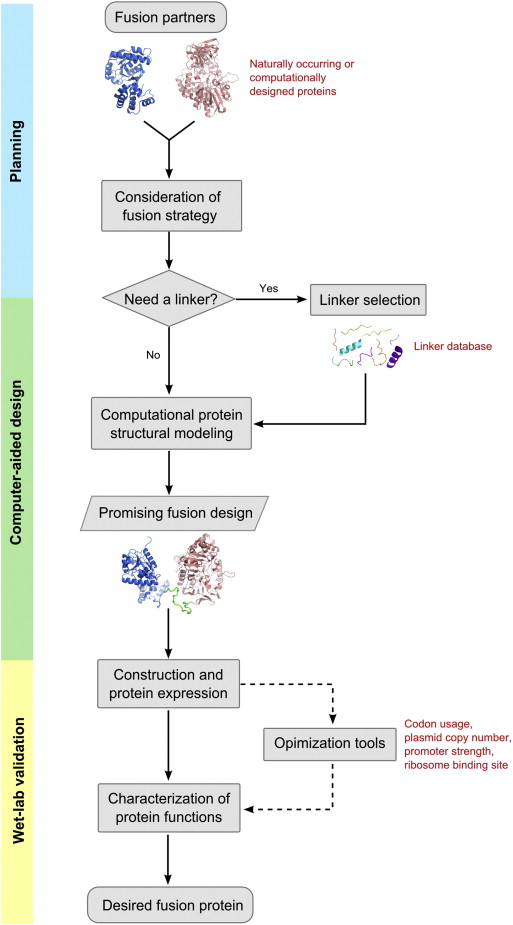
\includegraphics[width=140px]{../img/esquemaProcesoFusion.jpg}
% \end{center}
% \end{frame}






\begin{frame}{Relevant linker properties}
% Based on engineering process and linker function we can extract some properties
\begin{itemize}
%   BASED ON PREVOUSLY DEFINED FUNCTION
  \item Length
  \item Extended conformation
%   Lack of structure
% ya vimos que la estructura puede restringir los movimientos
%   \item Intrinsically disordered
%     \begin{itemize}
%     \item Extended conformation
%     \item Flexibility
%     \end{itemize}
  \item Biologically inert  %lack of functional features
  \item Other experimental aspects
    \begin{itemize}
     \item Aggregation, AAs frequencies, UV silent, net charge
%   Composition
    \end{itemize}
\end{itemize}
\pause
\vspace{15px}
%  Y CON TANTOS REQUERIMIENTOS..........
\Large{....linker design is not a trivial problem}
% \pause
% \\
% \vspace{10px}
% \huge{...one solution does \textbf{NOT} fits all.}
% we need to
\end{frame}



\begin{frame}{Linker design}
% SI QUEDA MUY GRANDE ESTA DIAPO LA PUEDO DIVIDIR EN 3 PARTES....!!!
% \pause
\begin{itemize}
 \item Use linkers from natural multi-domain proteins
 \pause
 \begin{itemize}
  \item structure?
  \item inert?
%  INCLUIR FIGURA!!!!

 \pause 
 \end{itemize}
 \item Intuitive design
%  there are lots of chimeric constructions that were experimentally tested....reuse. may involve small engineering process to adapt the sequence(lenght, composition, etc)
 \pause
 \begin{itemize}
  \item Reuse from literature or propose novel sequence. 
  \item Usually (G/S/P)-rich 
  \begin{itemize}
   \item  i.e $(GGGS)_n$ 
  \end{itemize}
  \item Very limited set of sequences and composition
  \end{itemize}
%  \pause
%  \subitem Requires experimental test (prueba y error) 

\end{itemize}
\end{frame}


\begin{frame}{Linker design}
%  \item Pseudo-Rational design
%   \pause 

  \begin{itemize}
    \item Pseudo-Rational design (LINKER, Linkerdb, SynLinker)
    \vspace{6px}
    \item DB (natural/previously used designs)
%     these include from different collections obtained in different projects	
\pause
    \Put(20,10){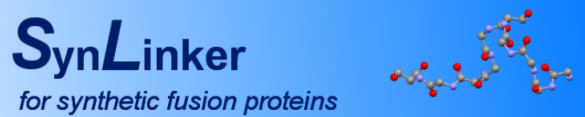
\includegraphics[width=100px]{../img/synLinkerLogo.png}}
 \end{itemize}

%  \item We cannot always get a solution %a suitable solution
% \end{itemize}

%  \vspace{10px}
%  \centering
\begin{adjustwidth}{-1em}{-2.5em}
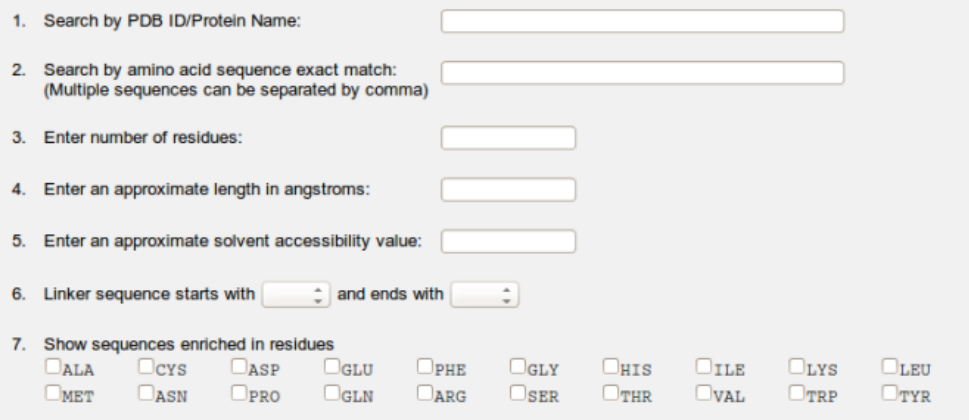
\includegraphics[width=330px]{../img/synLinker.png}
\end{adjustwidth}
% \begin{itemize}
%  \item Always applicable?
% \end{itemize}

\end{frame}









\section{Method}

\begin{frame}{Rational approach}
No method can provide a clean design\\ % a design clean of unwanted properties
\vspace{5px}
\pause
If we have a candidate linker sequence...
\pause
\begin{itemize}
\item Structural aspects $\rightarrow$ IUPred \pause
\item Functional aspects $\rightarrow$ BLAST, LMs, PROSITE, ANCHOR  \pause
\item Aggregation propensity $\rightarrow$ TANGO, PASTA  
\end{itemize}


% all apsects associated with linker properties can be assses by means of different bioinformatic tools available, that can analyze the sequence
% a pesar que los requerimientos no son muuchos, es decir, podemos asumir que gran cantidad de secuencias podrian funcionar como linkers

% We can evaluate (get an idea, get an estimation of) how good or how bad(quality) is a sequence to work as a linker.
% We can predict all unwanted properties.

\vspace{10px}
\pause 
\Large{Use this information to aid in linker design process}



% ESTO ES BASICAMENTE EL FUNDAMENTO DEL MÉTODO
% if we want to use this aspects to evaluate
% para usar esta informacion necesitamos 2 cosas
% 1 - formalize this estimation idea...i mean, we can get automatize and quantify the evaluation 
% AND
% 2 - find a good way to search for candidate sequences , to evaluate if they have the desired properties.
%	 we (probably) cant just start testing random sequences and see if they work...it would be highly inefficient
%	 we cant use natural sequences because, as we said, they dont always fulfill our needs
% 
% if we can find these 2 things we will have a design method
% 
% what is more, in our application these 2 aspects are connected !!!
\end{frame}



% ACA EXPLICO EL PUNTO 1 - CUANTIFICACION DE LA CALIDAD 
\begin{frame}{Linker evaluation}
\begin{itemize}

%  Turn the evaluation schema into a function $f(sequence) -> score$
% quantify using discrete values
 \item Turn the estimation into a scoring function by calculating the undesired features\\
% Penalize unwanted properties\\
% Quantify how good(or bad) is a sequence

% quantify de quality of the sequence
% es decir...if we define a function f(face)
%  \pause
%   \item Higher score $\rightarrow$ unwanted properties $\rightarrow$ worse linker
 \pause
 \item Score $\geqslant 0$ (Higher score $\rightarrow$ bad linker)
% we dont really care how high or low is the score, we want a linker with score = 0
\end{itemize}

% ES IMPORTANTE DESTACAR QUE EL PROCESO DE EVALUACIÓN CAN BE ADAPTED TO ANY RELEVANT ASPECT THAT WANT TO BE ASSESED
% IF YOU THINK THAT ITS GONNA BE RELEVANT THAT ASSES 
% \vspace{0.3cm}
% \begin{adjustwidth}{-1.5em}{-2.5em}
\pause
\begin{tabular}{llllllllllllll} 
\hline
Sequence & \textbf{M} & \textbf{V} & \textbf{L} & \textbf{S} & \textbf{P} & \textbf{A} & \textbf{D} & \textbf{K} & \textbf{T} & \textbf{N} & \textbf{P} & \textbf{D} \\ \hline \hline
\pause
% Puntaje Inicial & 0 & 0 & 0 & 0 & 0 & 0 & 0 & 0 & 0 & 0 & 0 & 0\\ \hline
IUPred                 & 0 & 1 & 1 & 1 & 1 & 0 & 1 & 1 & 1 & 1 & 0 & 0\\ \hline \pause
TANGO 		       & 1 & 1 & 1 & 1 & 0 & 0 & 0 & 0 & 0 & 0 & 0 & 0\\ \hline \pause
Linear motifs          & 1 & 1 & 1 & 1 & 0 & 0 & 0 & 0 & 0 & 1 & 1 & 1\\ \hline \pause
....                   & 2 & 1 & 1 & 1 & 1 & 0 & 3 & 2 & 5 & 4 & 1 & 0\\ \hline \hline
\pause
Position score         & 4 & 4 & 4 & 4 & 2 & 0 & 4 & 3 & 6 & 6 & 2 & 1\\ \hline
\pause
Global Score  & 40 \\ \hline
\end{tabular}
% \end{adjustwidth}
\end{frame}






% dijimos que queriamos usar esta informacion (el score) to aid in linker design
\begin{frame}{Linker design}
% the second thing we need is 
% ahora que definimos un score
\begin{itemize}
 \item Aiming at sequence with Global score = 0.
 \pause
 \item We have information for each position and the whole sequence
%  \item We have information of quality(score) at sequence level (detalied for each position).
\pause
\end{itemize}

%  TENEMOS INFORMACION SOBRE DETALLADA A NIVEL DE RESIDUO(NO SOLO EL SCORE GLOBAL)
% we can use this information to guide the search

% so, we propose a search method 
% We propose a search method: 
% to search for (optimal) sequence 
\begin{enumerate}
 \item Propose tentative linker as starting sequence 
%     \begin{itemize}
%     \item Random sequence works too! (\textit{de novo} design)
%     \end{itemize}
  \pause
 \item Propose point mutations to high scoring positions
%  we will get back to this later
      \begin{itemize}
      \item If score decreases $\rightarrow$ incorporate mutation to design.
      \item If NOT $\rightarrow$ heuristic decision (Score difference $\rightarrow$  $A_{rate}$).
     \end{itemize}
 \item Repeat step 2 until score=0
\end{enumerate}

\pause
Random sequences can work too! (\textit{de novo} design)\\
\pause
Obtaining a design is now an optimization problem


% and we are trying to apply an heuristic search method

% SOLVING AN OPTIMIZATION PROBLEM MIGHT HAVE DIFFERENT SOLUTIONS
% una aproximacion mediante mutaciones permitiria buscar soluciones similares a una secuencia inicial definida por el usuario
% ademas, mediante el control de la frecuencia de aminoacidos podriamos controlar la composicion

\end{frame}




\begin{frame}
\vspace{-0.5\baselineskip}
\begin{adjustwidth}{-1.5em}{-2.5em}
% \begin{adjustheight}{-1.5em}{-1.5em}
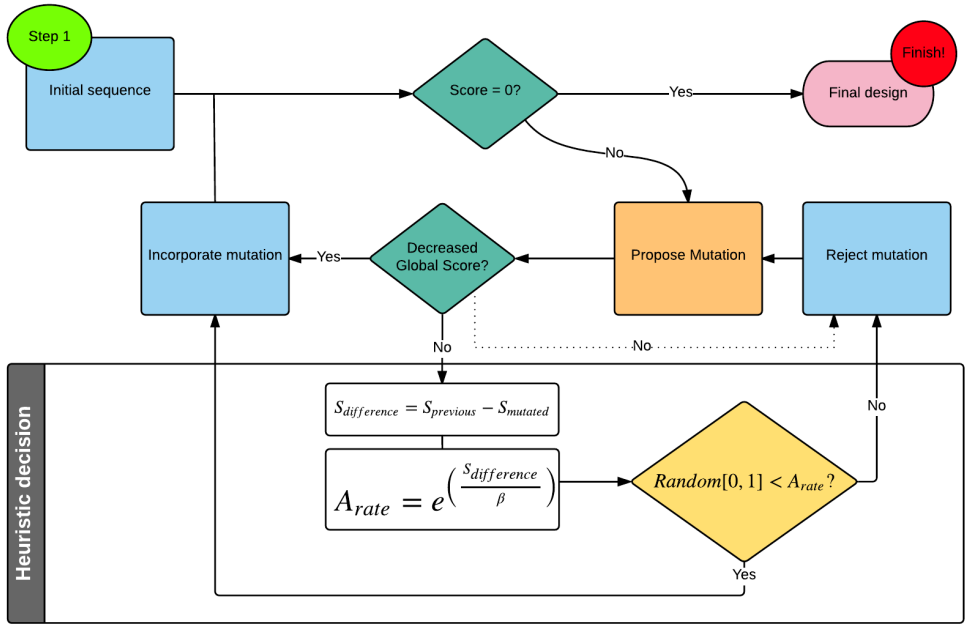
\includegraphics[width=340px,height=220px]{../img/patenaFixed.png} 
% \end{adjustheight}
\end{adjustwidth}
% \vspace{-\baselineskip}
\end{frame}





\section{Results}

\begin{frame}
% \vspace{-0.5\baselineskip}
\begin{adjustwidth}{-1.5em}{-2.5em}
\centering
% \begin{Verbatim}
How many mutations are required?  - \hspace{5px} Length = 30   
% Length = 30 residues \hspace{5px} - \hspace{5px}   Effect of $\beta$  
% \end{Verbatim}
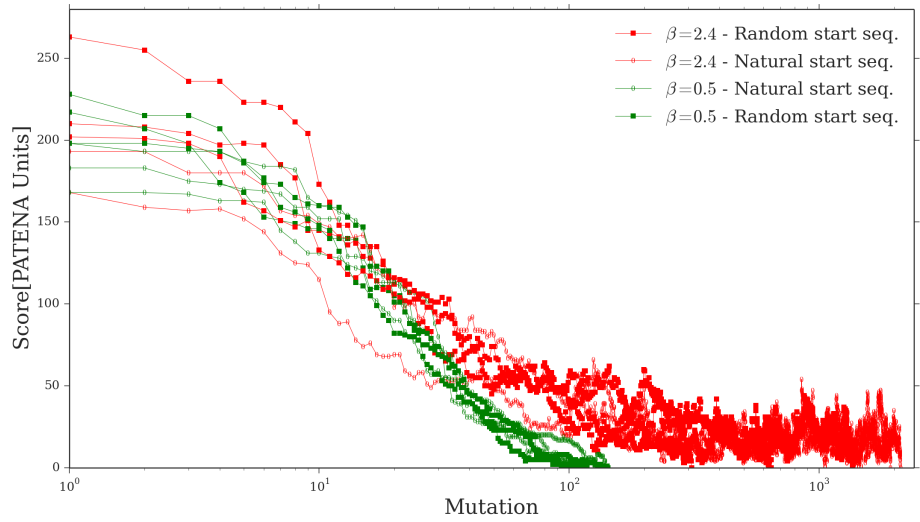
\includegraphics[width=330px,height=210px]{../img/scoreVsMutation-individual.png} 

\end{adjustwidth}
% \vspace{-\baselineskip}
\end{frame}


\begin{frame}
\centering
% Optimal $\beta$ range  
[Length = 50] - [Random (n=3) and Natural (n=3) seq. / each $\beta$] \\
\begin{adjustwidth}{-1.5em}{-2.5em}
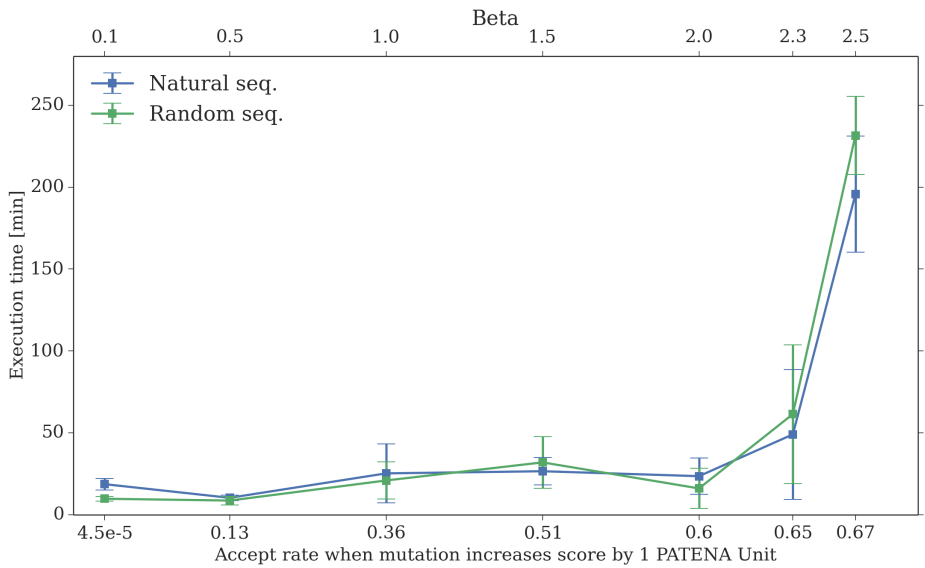
\includegraphics[width=330px,height=210px]{../img/betaVsTime.png} 
\end{adjustwidth}
\end{frame}


\begin{frame}
\centering
% Optimal $\beta$ range  
% [Length = 30] - [Random (n=3) and Natural (n=3) seq. / each $\beta$] \\
\begin{adjustwidth}{-1.5em}{-2.5em}
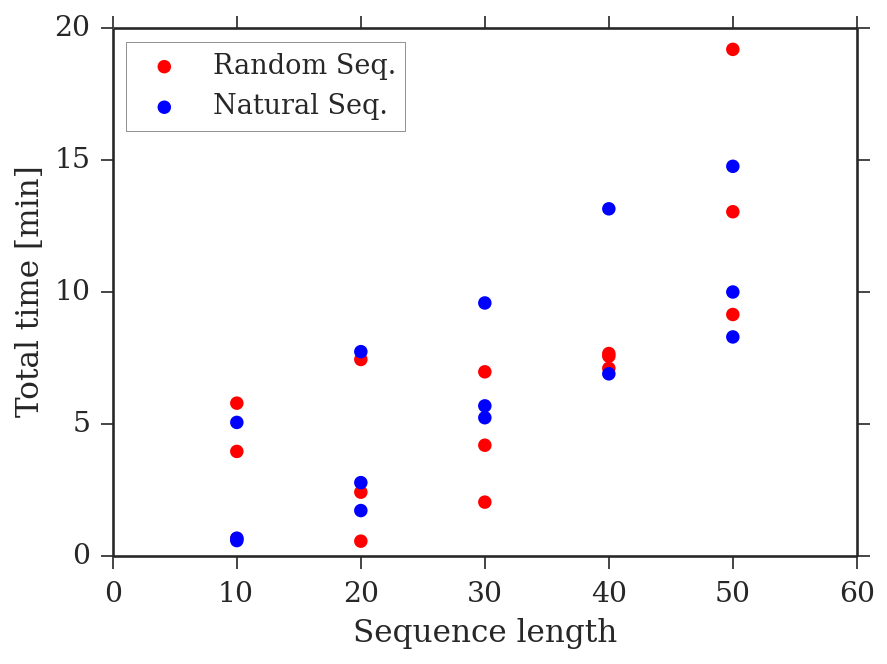
\includegraphics[width=330px,height=210px]{../img/lengthVsTime.png} 
\end{adjustwidth}
\end{frame}



\begin{frame}
\centering
Fixed starting sequence $\rightarrow$ 74 designs\\
\begin{adjustwidth}{-1.5em}{-2.5em}
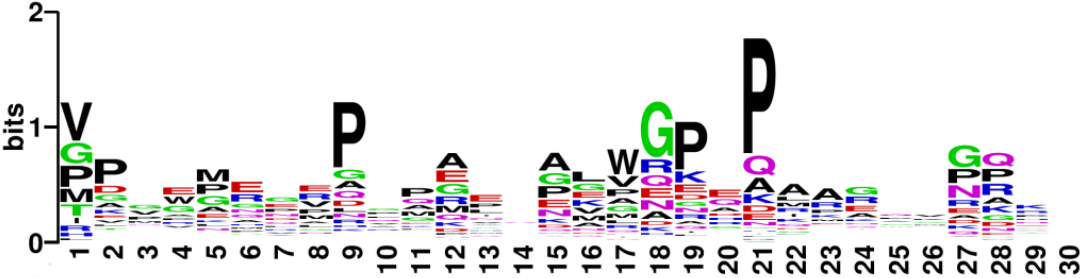
\includegraphics[width=340px,height=150px]{../img/logo.png}\\ 
\vspace{10px}
\hspace{18px}
\includegraphics[width=325px,height=15px]{../img/sequence.png}
\end{adjustwidth}
\end{frame}



\begin{frame}
\begin{adjustwidth}{-1.5em}{-2.5em}
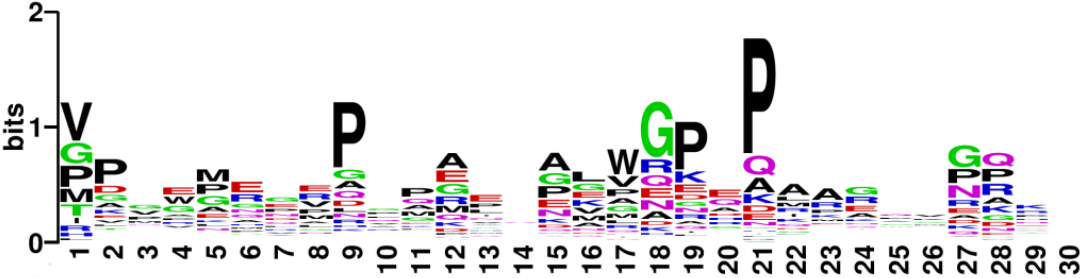
\includegraphics[width=340px,height=150px]{../img/logo.png}\\ 
% \vspace{10px}
\hspace{18px}
\includegraphics[width=325px,height=25px]{../img/sequence2.png}
\end{adjustwidth}
\end{frame}


\begin{frame}{Concluding remarks}
\begin{itemize}
 \item PATENA can find suitable protein linkers in a short execution time.
 \item The set of designs that can be obtained from the same sequence shows high diversity. 
 \item We interpret that the space of suitable linker sequences is a large fraction of the whole sequence space.
\end{itemize}
\end{frame}





% EXTRA


% Mutation attempts Vs Iter
\begin{frame}
\begin{adjustwidth}{-1.5em}{-2.5em}
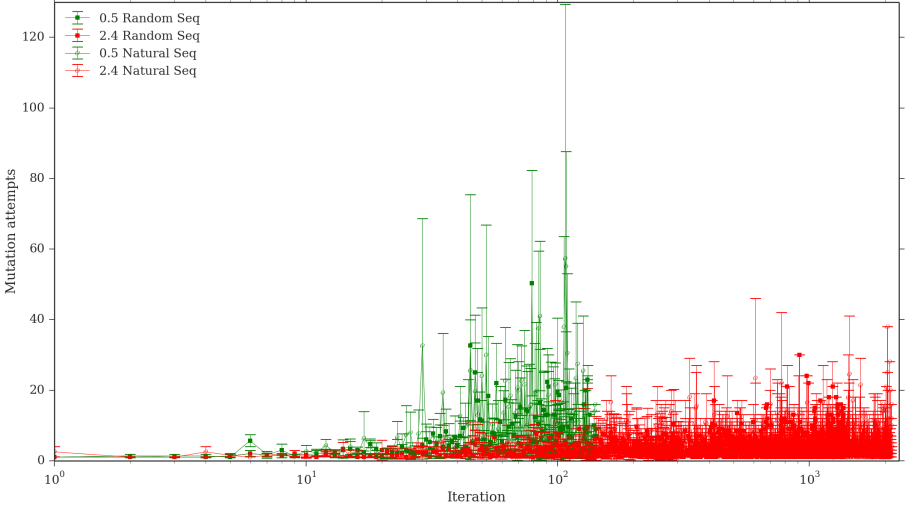
\includegraphics[width=340px,height=210px]{../img/mutAttemptsVsMutation.png} 
\end{adjustwidth}
\end{frame}

\begin{frame}
\begin{adjustwidth}{-1.5em}{-2.5em}
Fixed starting sequence $\rightarrow$ 74 designs\\
\vspace{15px}
\hspace{10px} Identity between resulting designs  \hspace{15px}   Identity against starting seq.
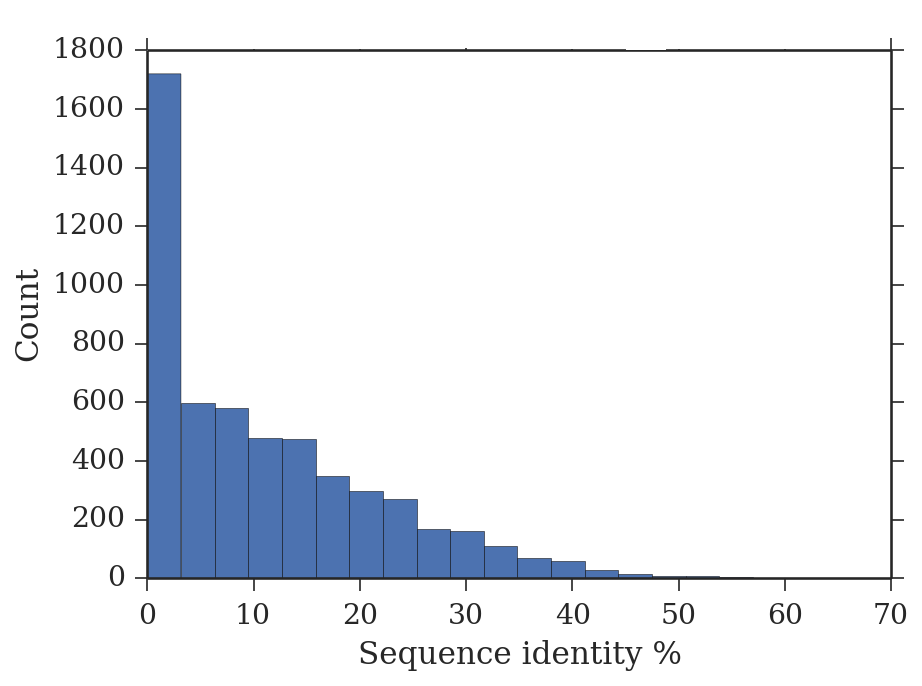
\includegraphics[width=175px,height=145px]{../img/againstAll.png}
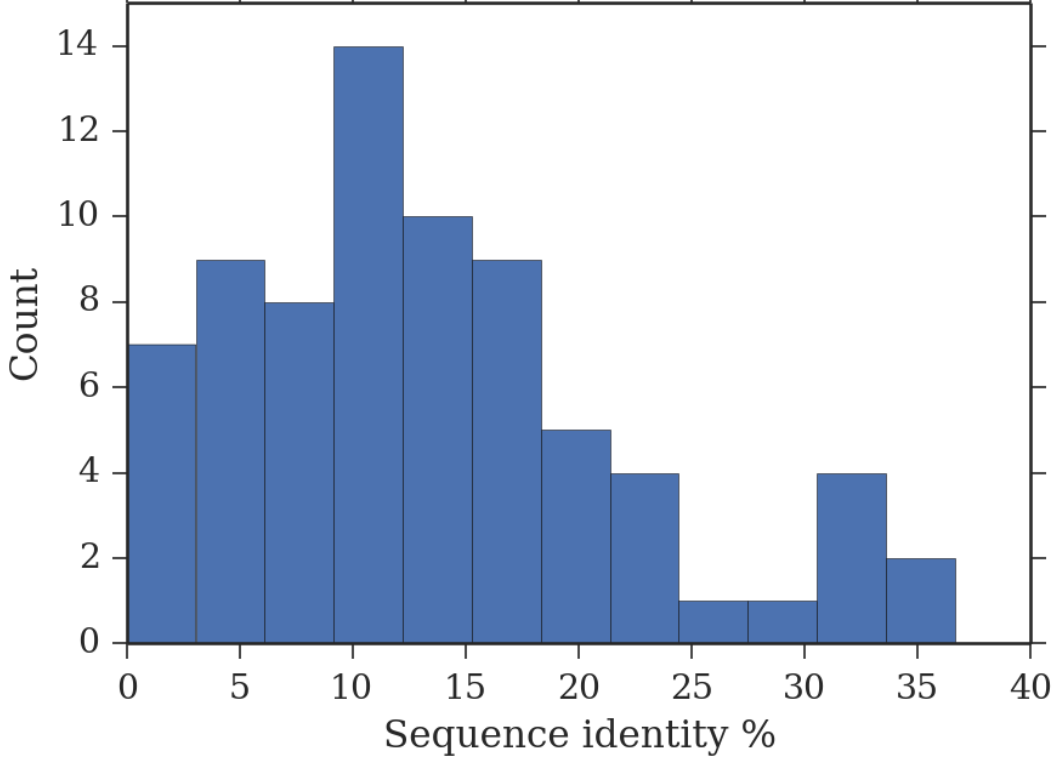
\includegraphics[width=160px,height=135px]{../img/againstStartSeq.png}
\end{adjustwidth}
\end{frame}



\begin{frame}
\centering
Fixed starting sequence $\rightarrow$ 74 designs \\
\begin{adjustwidth}{-1.5em}{-2.5em}
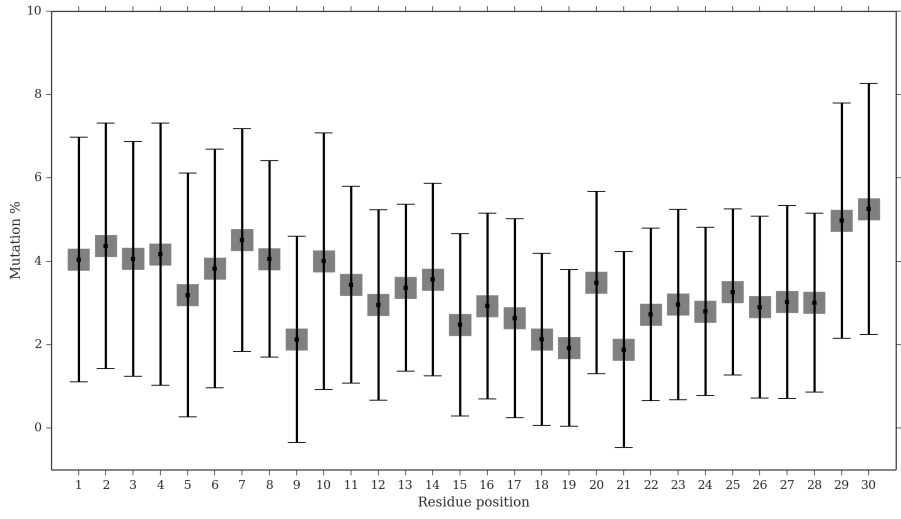
\includegraphics[width=340px,height=150px]{../img/mutationsPerPosition.png}\\ 
% \vspace{10px}
\hspace{25px}
\includegraphics[width=310px,height=10px]{../img/sequence.png}
\end{adjustwidth}
\end{frame}


\begin{frame}
\centering
Fixed starting sequence $\rightarrow$ 74 designs - Beta 0.5 , 0.1\\

\begin{adjustwidth}{-1.5em}{-2.5em}
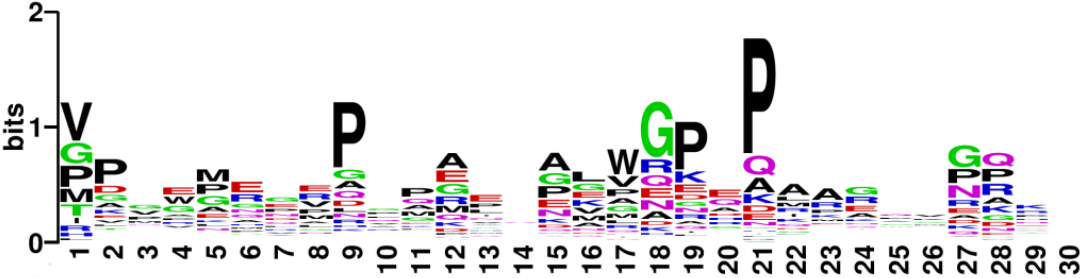
\includegraphics[width=340px,height=80px]{../img/logo.png}\\ 
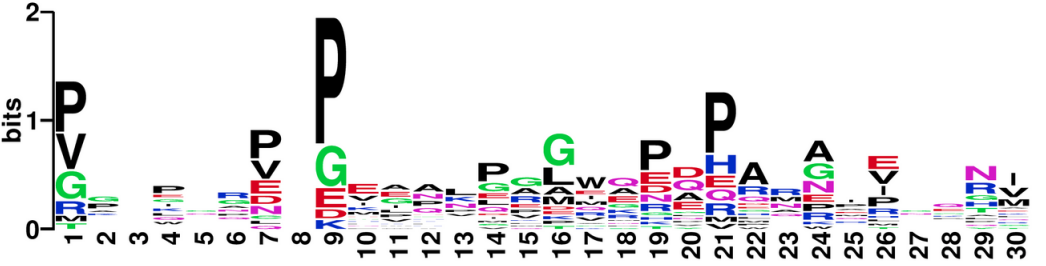
\includegraphics[width=345px,height=80px]{../img/logoBeta0-1.png}\\ 
\vspace{5px}
\hspace{18px}
\includegraphics[width=324px,height=15px]{../img/sequence.png}
\end{adjustwidth}
\end{frame}

\end{document}
